
First we can find the lines at a distance of 4 from the given line and then it's intersection with the x-axis.


\[\textbf{n}=\myvec{-4 \\ 3}\]

The parallel lines must have the same slope but different intercepts. Hence the lines must be of the form:

\begin{align}
\myvec{4 & 3} \vec{x} = {c_1} 
\\
\myvec{4 & 3} \vec{x} = {c_2}
\end{align}
These $c_1$ and $c_2$ can be easily found by evaluating the distance between the parallel lines:
\begin{align}
\frac{\abs{( c - 12 )}}{\sqrt{4^{2} + 3^{2}}} = 4
\end{align}
\begin{align}
c = 12 \pm 20
\end{align}


The two parallel lines at a distance of 4 thus obtained are:

\begin{align}
\myvec{4 & 3}\vec{x} = 32
\\
\myvec{4 & 3}\vec{x} = -8
\end{align}
Finally the points on x-axis are:
\begin{align}
\vec{x} = 8
\\
\vec{x} = -2
\end{align}

See Fig. \ref{fig1:solutions/line_plane/34/}


\begin{figure}[!ht]

\centering

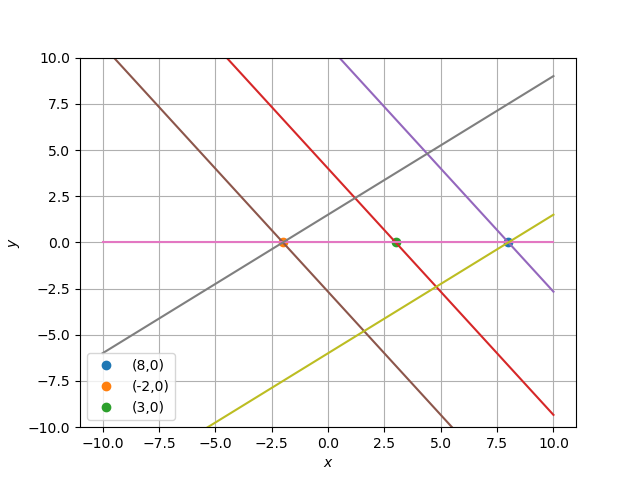
\includegraphics[width=\columnwidth]{./solutions/line_plane/34/figs/Figure_1.png}

\caption{Points on x-axis at a distance of 4 from the given line}

\label{fig1:solutions/line_plane/34/}

\end{figure}
